\chapter{Numerical model for vegetation in urban areas}
\label{ch:numericalmethod}
\def\figdir{chapters/ch07_numericalmodel/figures}	

\section{Introduction}

\lettrine[lines=3,nindent=0em,loversize=0.1]{T}{he} simplified vegetation model is described in \cref{ch:parametricstudy} introduction the governing equation for moist flow vegetation. The vegetation model provides the necessary source/sink terms for heat, mass and momentum exchanges between vegetation and air as described in \cref{sec:cons_incompressible}. Furthermore, radiation transfer within vegetation is also described in \cref{sec:vegradiation}. For reader, a detailed derivation of the thermodynamic of the moist air is given in \cref{app:thermodynamics} and a detailed derivation of the governing equation of moist flow is given in \cref{app:conservation}. 

In this chapter, the numerical method for modeling vegetation inside an urban area is described. The chapter focuses on coupling of the vegetation model with the of heat (incl. radiation) and mass fluxes of the urban surfaces. The governing  equation for the the coupled heat and moisture transport in the porous material is first described.

\section{Governing equations of coupled heat and moisture transport}

\subsection{Composition of the porous material}

The building materials and the soil is considered as a porous material consisting of three phases: solid phase (denoted with $s$), liquid phase referring to liquid water ($l$) and the air phase which is split into dry air ($a$) and water vapor $v$ \citep{Defraeye2011, Saneinejad2013, Carmeliet2005,Janssen2002}. The open porosity $\phi_o$ (m$^3$\,m$^{-3}$) of the porous material is defined as:
\begin{equation}
\phi_o = \frac{V_{\mathit{pore}}}{V}
\end{equation}
where $V_{\textit{pore}}$ (m$^3$) is the volume of open pores and $V$ (m$^3$) is the total volume of the porous material $\tensor{S}$. The solid material content $w_s$ (kg\,m$^{-3}$) is defined as:
\begin{equation}
w_s = \left(1 - \phi_o \right) \rho_s
\end{equation}
where $\rho_s$ (kg\,m$^{-3}$) is the solid material matrix density. Similarly the dry air $w_a$, water vapor $w_v$, liquid water $w_l$ contents are defined as:
\begin{align}
w_l &= \phi_o S_l \rho_l \\
w_a &= \phi_o \left( 1 - S_l \right) \rho_a \\
w_v &= \phi_o \left( 1 - S_l \right) \rho_v
\end{align}
where they are related to the degree of liquid saturation $S_l$ of the porous open pores:
\begin{equation}
S_l = \frac{\phi_{\textit{o,l}}}{\phi_o}
\end{equation}
with $\phi_{\textit{o,l}}$ being the amount of liquid water occupied inside the open pores and $\rho_a$, $\rho_l$ being the air and liquid water densities, respectively. The total moisture content $w$ (kg\,m$^{-3}$) inside the porous material is simply the sum of liquid water and water vapor:
\begin{equation}
w = w_l + w_v
\end{equation}

\subsection{Water potential}

Water potential is a universal parameter to determine the \textit{water status} in any medium \citep{nobel2009physicochemical}. In the thesis, we use it to define the water status of multiple domains such as solid porous materials (soil and building facades), plant xylem, and air. The water potential $\psi$ (Pa) describes the chemical potential of water $\mu$ (J\,mol$^{-1}$) with respect to chemical potential of pure water $\mu^{o,l}$ (J\,mol$^{-1}$) at the same temperature, standard atmosphere and at zero level:
\begin{equation}
\psi = \frac{\mu - \mu^{o,l}}{V^o_l}
\end{equation}
where $V^o_l = 18.05 \num{e-3}$ m$^3$\,mol$^{-1}$ is the molar volume of pure water in liquid phase. The water potential for pure water at standard atmosphere is $\psi = 0$ Pa. The water tends to move towards a region where $\mu-\mu^{o_w}$ is lower, i.e. in the direction of $-\nabla\psi$. The water potential is related to pressure potential, osmotic potential, matrix potential, and gravitational potential. In our study, we assume that the pressure potential gradient is negligible in the solid and we ignore the influence of osmotic potential $\psi_o$ (Pa) as we assume we have a non-saline porous material. Therefore, only the matrix potential and gravitation potential influences the water transport:
\begin{equation}
\psi = \underbrace{p_c}_{\psi_c} + \underbrace{\rho_l g z}_{\psi_g}
\end{equation}
where $\psi_c = p_c$ (Pa) is the capillary potential due to capillary pressure, which represents the contribution of the matrix potential, and $\psi_g = \rho_l g h$ (Pa) is the gravitational potential with $g = |\mvec{g}|$ (m\,s$^{-2}$) where $\mvec{g}$ is the gravitational acceleration. The capillary pressure $p_c$ is defined as the difference between liquid and gas phase pressure, $p_l$ and $p_g$, respectively:
\begin{equation}
p_c =  p_l - p_g
\end{equation}
and is related to relative humidity $\phi$ by the Kelvin's law:
\begin{equation}
p_c = \rho_l R_v T \ln \left(\phi\right)
\end{equation}

The gravitational potential $\psi_g$ (Pa) is defined as:
\begin{equation}
\psi_g = - \rho \mvec{g} \cdot \mvec{x} = \rho g z
\end{equation}
where $g = |\mvec{g}|$ with $z$ oriented upward. Thus, by taking the capillary and gravitational water potentials into account, the transport of water can be described in building materials and, more importantly, soil where the plant roots are present.

\subsection{Coupled transport of heat and mass}

The conservation of mass in the solid domain is defined as:
\begin{align}
\pde{w_s}{t} &= 0 \label{eq:solidcom} \\ 
\pde{w_a}{t} + \nabla \cdot \left(w_a\mvec{u}_a \right) &= 0 \label{eq:aircom} \\ 
\pde{w_l + w_v}{t} + \nabla \cdot \left(w_l\mvec{u}_l + w_v\mvec{u}_v \right) &= 0 \label{eq:liqcom}
\end{align}
assuming that solid matrix does not move, mass of different phases only change due to evaporation or condensation. Other phenomena such as melting, freezing, sublimation and deposition are neglected. As we are only interested in the rate of change of moisture content $w = w_l + w_g$, we are only interested in \cref{eq:liqcom} and conservation of mass simplifies to:
\begin{equation}
 \pde{w}{t} = - \nabla \cdot \left(\mvec{g}_l + \mvec{g}_v \right)
\end{equation}
where $\mvec{g}_l \equiv w_l\mvec{u}_l$ (kg\,m$^{-2}$\,s$^{-1}$) and $\mvec{g}_v \equiv w_v\mvec{u}_v$ (kg\,m$^{-2}$\,s$^{-1}$) are defined as the liquid water and water vapor fluxes, respectively. Additionally, the contribution of root water uptake due to plant transpiration is introduced through the source term $s_r$ (kg\,m$^{-3}$\,s$^{-1}$):
\begin{equation}
\pde{w}{t} = - \nabla \cdot \left(\mvec{g}_l + \mvec{g}_v \right) + s_r
\label{eq:com4}
\end{equation}

The sink term due to root water uptake is explained in detail later in \cref{sec:spac}. In this thesis, the conservation of mass is solved using the $p_c$-form Richards equation, where \cref{eq:com4} becomes:
\begin{equation}
\frac{\partial w}{\partial p_c} \frac{\partial p_c}{\partial t} = -  \nabla \cdot \left(\mvec{g}_l + \mvec{g}_v\right) + s_{r}
\label{eq:com5}
\end{equation}
with $C_{mm} \equiv \partial w/ \partial p_c$ (kg\,m$^{-3}$\,Pa$^{-1}$) is defined as the moisture capacity. Thus, the change in water content in the porous material is simply due to the liquid and vapor fluxes, and root water uptake. The liquid water flux $\mvec{g}_l$ in porous media is given by:
\begin{equation}
\mvec{g}_l = - K_{\textit{lp}} \nabla \left(p_c + \rho_l g z\right)
\label{eq:liquidflux}
\end{equation}
and assumes the air pressure effects be negligible with respect to capillary and gravitational effects, where $K_{\textit{lp}}$ (s) the liquid water permeability. We assume that the liquid water permeability is only due to pressure gradient, and the influence of thermal gradient is neglected \citep{Carmeliet2005}. The water vapor flux in the porous media is given by:
\begin{equation}
\mvec{g}_v = K_{\textit{vp}}\nabla p_c + K_{\textit{vT}}\nabla T
\label{eq:vaporflux}
\end{equation}
where
\begin{equation}
K_{\textit{vp}} = - \delta_v \frac{p_v}{\rho_l R_v T}
\end{equation}
is the water vapor permeability (s) due to pressure,  
\begin{equation}
K_{\textit{vT}} = - \delta_v \frac{p_v}{\rho_l R_v T^2}\left(\rho_l L_v - p_c\right)
\end{equation}
is the water vapor permeability (s) due to temperature, and
\begin{equation}
\delta_v = \frac{D_{\textit{va,mat}}}{R_v T}
\end{equation}
is the water vapor diffusion coefficient (s) where $D_{\textit{va,mat}}$ (m$^2$\,s$^{-1}$) is the binary apparent diffusion coefficient between dry air and water vapor \citep{Carmeliet2005, Defraeye2011, Saneinejad2013, Kubilay2014b}. Thus, substituting the fluxes \cref{eq:liquidflux,eq:vaporflux} into \cref{eq:com5}, the expanded form of conservation of mass is given as:
\begin{equation}
C_{\textit{mm}}\frac{\partial p_c}{\partial t} = \nabla \cdot \Big( K_{lp} \nabla \left(p_c + \rho_l g z\right) + K_{\textit{vp}}\nabla p_c + K_{\textit{vT}}\nabla T \Big) + s_r
\label{eq:com6}
\end{equation}

The conservation of energy is given as:
\begin{equation}
\frac{\partial h}{\partial t} + \nabla \cdot \left(h \mvec{u}\right) = - \nabla \cdot \mvec{q}
\label{eq:coe1}
\end{equation}
where $h$ (J\,kg$^{-1}$) is the enthalpy of total solid domain:
\begin{equation}
h = \sum_i w_i h_i = w_s h_s + w_a h_a + w_l h_l + w_v h_v
\label{eq:enthalphy1}
\end{equation}
assuming that thermal contribution of soil and liquid water is much higher than dry air and water vapor. The heat conduction $\mvec{q}$ (W\,m$^{-2}$) is given by Fourier's law as:
\begin{equation}
\mvec{q} = -\lambda \nabla T
\label{eq:fourierlaw}
\end{equation}
where $T$ (K) is temperature, $\lambda$ (W\,m$^{-1}$\,K$^{-1}$) is thermal conductivity. Substituting \cref{eq:enthalphy1} into \cref{eq:coe1} gives:
\begin{equation}
\frac{\partial}{\partial t}\left(w_s h_s + w_l h_l\right) = - \nabla \cdot \mvec{q} - \nabla \cdot \left(w_l h_l \mvec{u}_l + w_v h_v \mvec{u}_v\right)
\end{equation}
or equivalently written as:
\begin{equation}
\frac{\partial}{\partial t}\left(w_s h_s + w_l h_l\right) = - \nabla \cdot \mvec{q} - \nabla \cdot \left(h_l \mvec{g}_l + h_v \mvec{g}_v\right)
\label{eq:coe2}
\end{equation}
where the enthalpy of liquid water $h_l$ and water vapor $h_v$ are defined as:
\begin{align}
h_l &= c_{p,l} \left(T - T_{\textit{ref}}\right) \label{eq:enthalphyl}\\
h_v &= c_{p,v} \left(T - T_{\textit{ref}}\right) + L_v \label{eq:enthalphyv}
\end{align}
and $L_v$ is the latent heat of vaporization of water. Substituting \cref{eq:enthalphyl,eq:enthalphyv} into \cref{eq:coe2}, the conservation of energy is given as:
\begin{equation}
\begin{split}
&\left(c_{\textit{ps}} w_s + c_{\textit{pl}} w\right)\frac{\partial T}{\partial t} + \left[c_{pl} \left(T - T_{\textit{ref}}\right) \frac{\partial w}{p_c}\right]\frac{\partial p_c}{\partial t} =\\
& - \nabla \cdot \bigg\{ {\mvec{q} + \underbrace{ c_{\textit{pl}} \left(T - T_{\textit{ref}}\right)\mvec{g}_l}_{\mvec{q}_l} + \underbrace{ \Big[c_{\textit{pv}} \left(T - T_{\textit{ref}}\right) + L_v\Big]\mvec{g}_v}_{\mvec{q}_v} } \bigg\}
\end{split}
\label{eq:coe3}
\end{equation}
where the capacity terms are:
\begin{align}
C_{\textit{TT}} &=  c_{\textit{ps}}w_s + c_{\textit{pl}}w \label{eq:cap1} \\
C_{\textit{Tp}} &=  c_{\textit{pl}} \left( T - T_{\mathit{ref}}\right) \pde{w}{p_c} \label{eq:cap2} 
\end{align}

Substituting liquid and vapour fluxes, \cref{eq:liquidflux,eq:vaporflux}, respectively, thermal capacities \cref{eq:cap1,eq:cap2} and heat conduction \cref{eq:fourierlaw} into conservation of energy expands \cref{eq:coe3} to:
\begin{align}
\begin{aligned}
		\mathllap{C_{\textit{TT}}\frac{\partial T}{\partial t} + C_{\textit{Tp}}\frac{\partial p_c}{\partial t}} = \nabla \cdot \bigg(\lambda \nabla T &+  K_{\textit{lp}} c_{\textit{pl}} \left(T - T_{\textit{ref}}\right)  \nabla p_c \\
					&+ K_{\textit{lp}} c_{\textit{pl}} \left(T - T_{\textit{ref}}\right) \rho_l g z\\
					&- K_{\textit{vp}} \Big[c_{\textit{pv}} \left(T - T_{\textit{ref}}\right) + L_v\Big] \nabla p_c \\ 
					&- K_{\textit{vT}} \Big[c_{\textit{pv}} \left(T - T_{\textit{ref}}\right) + L_v\Big] \nabla T \bigg)
\end{aligned}
\end{align}

\subsection{Linearized heat and mass transport equation}
In the present study, the conservation of mass and energy is coupled together as a heat and mass model (HAM) according to \citep{Janssen2002,Defraeye2011,Carmeliet2005,Saneinejad2013,Kubilay2018}. Due to the shape of the water retention curve and the hydraulic conductivity curve, the Richards equation is highly non-linear as shown in .

\begin{figure}[h]
	\centering
	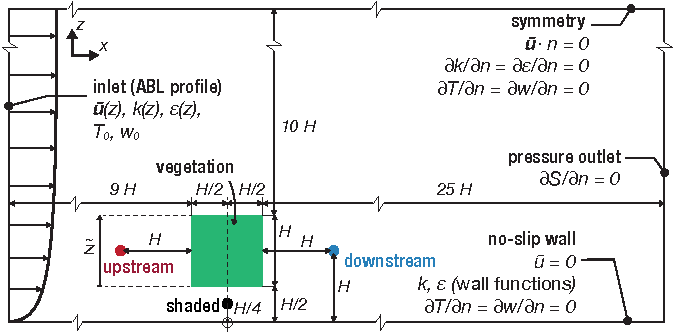
\includegraphics[width=\textwidth]{\figdir/domain-crop.pdf}
	\caption{}
	\label{fig:domain}
\end{figure}



Therefore, the numerical solution of the equation is very sensitive to convergence tolerance and requires linearization techniques to maintain accuracy and computational efficiency. Therefore, methods such as fixed-point Picard iterations is used to solve the non-linear equations. More details on the discretization is provided in \cite{Liu2012,Janssen2002,Kubilay2018}. The conservation of mass (i.e., the moisture transport equation), \cref{eq:com6}, in the linearized form is given as:
\begin{equation}
\begin{split}
C^{n+1,k}_{\textit{mm}}\frac{p_c^{n+1,k+1}-p_c^{n}}{\Delta t} = \nabla \cdot \Big( K_{\textit{lp}}^{n+1,k} &\nabla \left(p_c^{n+1,k+1} + \rho_l g z\right)\\
&+ K_{\textit{vp}}^{n+1,k} \nabla p_c^{n+1,k+1} \\
&+ K_{vT}^{n+1,k} \nabla T^{n+1,k}\Big)\\
+ s_r^{n+1,k+1}&
\end{split}
\end{equation}
where the capacity, permeabilities and temperature are determined from the previous Picard iteration ($k$). The subscript ($n$) denotes the global (i.e., outer) time step of $t$ and $k$ denoting the internal Picard iteration step. When the Picard solution approaches converges, $p_c^{n+1,k} \rightarrow p_c^{n+1,k+1}$ and the influence of $\partial{w}/\partial p_c$ becomes negligible. This can results in larger mass conservation errors and can be minimized by using mixed-from:
\begin{equation}
\begin{split}
C^{n+1,k}_{\textit{mm}}\frac{p_c^{n+1,k+1}-p_c^{n}}{\Delta t} = \nabla \cdot \Big( K_{\textit{lp}}^{n+1,k} &\nabla \left(p_c^{n+1,k+1} + \rho_l g z\right)\\
&+ K_{\textit{vp}}^{n+1,k} \nabla p_c^{n+1,k+1} \\
&+ K_{vT}^{n+1,k} \nabla T^{n+1,k}\Big)\\
+ s_r^{n+1,k+1} &- \frac{w^{n+1,k+1}-w^n}{\Delta t}
\end{split}
\end{equation}

Similarly, the linearized form of the heat equation is defined as:
\begin{equation}
\begin{split}
	C_{\textit{TT}}^{n+1,k}& \frac{T^{n+1,k+1}-T^{n}}{\Delta t} = \nabla \cdot \bigg(\lambda \nabla T^{n+1,k+1} \\
	&+ K_{\textit{lp}}^{n+1,k} c_{\textit{pl}} \left(T^{n+1,k+1} - T_{\textit{ref}}\right)  \nabla p_c^{n+1,k+1} \\
	&+ K_{\textit{lp}}^{n+1,k} c_{\textit{pl}} \left(T^{n+1,k+1} - T_{\textit{ref}}\right) \rho_l g z\\
	&- K_{\textit{vp}}^{n+1,k} \Big[c_{\textit{pv}} \left(T^{n+1,k+1} - T_{\textit{ref}}\right) + L_v\Big] \nabla p_c^{n+1,k} \\ 
	&- K_{\textit{vT}}^{n+1,k} \Big[c_{\textit{pv}} \left(T^{n+1,k+1} - T_{\textit{ref}}\right) + L_v\Big] \nabla T^{n+1,k+1} \bigg)
\end{split}
\end{equation}
where the capillary pressure time derivative term is ignored. The mixed-form the heat equation is given as:
\begin{equation}
\begin{split}
C_{\textit{TT}}^{n+1,k}&\frac{T^{n+1,k+1}-T^{n}}{\Delta t} = \nabla \cdot \bigg(\lambda \nabla T^{n+1,k+1} \\
&+ K_{\textit{lp}}^{n+1,k} c_{\textit{pl}} \left(T^{n+1,k+1} - T_{\textit{ref}}\right)  \nabla p_c^{n+1,k+1} \\
&+ K_{\textit{lp}}^{n+1,k} c_{\textit{pl}} \left(T^{n+1,k+1} - T_{\textit{ref}}\right) \rho_l g z\\
&- K_{\textit{vp}}^{n+1,k} \Big[c_{\textit{pv}} \left(T^{n+1,k+1} - T_{\textit{ref}}\right) + L_v\Big] \nabla p_c^{n+1,k} \\
&- K_{\textit{vT}}^{n+1,k} \Big[c_{\textit{pv}} \left(T^{n+1,k+1} - T_{\textit{ref}}\right) + L_v\Big] \nabla T^{n+1,k+1} \bigg)\\
&- \frac{C_{TT}^{n+1}T^{n+1} - C_{TT}^{n}T^{n}}{\Delta t}
\end{split}
\end{equation}


The system of linear equations is solved by Krylov subspace iteration solver, i.e. preconditioned conjugate gradient (PCG) with diagonal-based incomplete Cholesky (DIG) preconditioning. The convergence criteria for the Picard iteration is user-defined: 
\begin{equation}
\left| p_c^{n+1,k+1} - p_c^{n+1,k}\right| \le \delta p_c
\end{equation}
\begin{equation}
\left| T^{n+1,k+1} - T^{n+1,k}\right| \le \delta T
\end{equation}
where $\delta p_c = \delta T = 10^{-2}$.

\section{Soil-Plant-Atmospheric Continuum}
\label{sec:spac}

In the present study, the components of the water potential inside the plants are not directly determined. The soil-plant-atmosphere continuum model that is integrated into the vegetation model is described in this section, implemented according the state-of-art techniques: \citep{Volpe2013,Manoli2014,Launiainen2015,Idso1977,Manzoni2011,Farquhar1980}. The root-system of the plants are represented as a network-like structure assuming cooperative strategy among the individual roots and a bulk plant transpiration through a single xylem is assumed.

\subsection{Water transport in soil-root system}

The hydraulic conductivity in soil $K$ (m\,s$^{-1}$) is given as:
\begin{equation}
K(\mvec{x}) = K_{\textit{lp}}(\mvec{x}) ~ |\mvec{g}|
\end{equation}
where $K_l$ (s) is the liquid permeability defined in the previous section and function on the moisture content. The soil conductance in the root region $k_s$ (s$^{-1}$) is:
\begin{equation}
k_s(\mvec{x}) = \alpha ~ K(\mvec{x}) ~ r(\mvec{x})
\end{equation}
where $\alpha$ is 
\begin{equation}
\alpha =  \sqrt{\left(\frac{L}{\textit{RAI}}\right) \frac{1}{d}}
\end{equation}
and $d$ is the root diameter and $\textit{RAI} = \int r~\mathrm{d}z$ is the root area index (m$^2$\,m$^{-2}$) and is the vertical integral of the root area density $r$ (m$^{2}$\,m$^{-3}$). The conductance of the root system $k_r$ (s$^{-1}$) is given as:
\begin{equation}
k_r(\mvec{x}) = r(\mvec{x})\frac{\Delta z}{\beta}
\end{equation}
where $\Delta z$ is the vertical height of the root layer mesh and $\beta = \num{3e8}$ s. The effective conductance of the soil-root system (or rhizosphere) $k_{sr}^*$ (s\,m$^{-1}$) is given as:
\begin{equation}
k_{sr}^*\left(\mvec{x}\right)  = \frac{1}{|\mvec{g}|} \frac{k_s\left(\mvec{x}\right)  k_r\left(\mvec{x}\right) }{k_s\left(\mvec{x}\right)  + k_r\left(\mvec{x}\right) }
\end{equation}

The sink in soil moisture $s_r$ (kg\,m$^{-3}$\,s$^{-1}$) is given as:
\begin{equation}
s_r(\mvec{x})  = r(\mvec{x}) ~ g_{v,root}(\mvec{x})
\end{equation}
where $g_{v,root}$ is the root water uptake (kg\,m$^{-2}$\,s$^{-1}$)
\begin{equation}
g_{v,root}(\mvec{x})  = k_{sr}^*(\mvec{x})  \left(\psi_s(\mvec{x})  - \psi_R\right)
\end{equation}
and simply dependent on the soil-root system conductance, soil water potential $\psi_s$ and the (bulk) root water potential $\psi_R$. The resulting net sink is soil moisture $G_{\textit{v,root}}$ (kg\,s$^{-1}$) due to transpiration is thus:
\begin{equation}
G_{\textit{v,root}} = \int_{\Omega_s} r(\mvec{x}) g_{v,root}(\mvec{x})~\mathrm{d}V
\end{equation}
where $\Omega_s$ is the soil domain. The water uptake from the root is equal to the water transport in the xylem as so:
\begin{equation}
G_{\textit{v,root}} = G_{\textit{v,xylem}}
\end{equation}

\subsection{Water transport in xylem-leaf system}

The plant xylem conductance is modeled using a ``\textit{vulnerability curve}'' approach, where xylem conductance becomes exponentially smaller with increasing leaf water potential \citep{Volpe2013}. This empirical model is based on plant response to the vulnerability to xylem cavitation and embolism that could occur at high water potential gradients. The xylem conductance $k_x$ (m\,Pa$^{-1}$\,s$^{-1}$) is given by:
\begin{equation}
k_x(\psi_L) = k_{\textit{x,max}} \exp \left\{ - \left( - \frac{\psi_L}{d}\right)^c \right\}
\end{equation}
where $k_{\textit{x,max}}$ (m\,Pa$^{-1}$\,s$^{-1}$) is the maximum xylem conductance, $c$ and $d$ are fit coefficients \citep{Volpe2013}, and $\psi_L$ (Pa) is the (bulk) leaf water potential. The effective xylem conductance $k_x^*$ (s\,m$^{-1}$) of water is:
\begin{equation}
k_x^* (\psi_L)= k_x(\psi_L) ~ \rho_l
\end{equation}
Thus, the water flux though the plant in xylem $g_{\textit{v,xylem}}$ (kg\,m$^{-2}$\,s$^{-1}$) is given as:
\begin{equation}
g_{\textit{v,xylem}}(\psi_L) = k_x^* \left(\psi_R - \psi_L\right)
\end{equation}
where is governed by the water potential gradient. The net water flux $G_{\textit{v,xylem}}$  (kg\,s$^{-1}$) is given as:
\begin{equation}   
G_{\textit{v,xylem}}(\psi_L) = \int_{\partial\Omega_{x|s}} g_{\textit{v,xylem}}(\psi_L)~\mathrm{d}A = g_{\textit{v,xylem}} A_x
\end{equation}
where $A_x$ (m$^2$) is the xylem cross-sectional area, assuming that the net water flux through the xylem is equal (i.e. no water storage).

Similarly, the net flux of water in xylem should be equal to the net transpiration rate, as storage is negligible. Therefore, 
\begin{equation}
G_{\textit{v,xylem}} = G_{\textit{v,leaf}}
\end{equation}
and moreover,
\begin{equation}
G_{\textit{v,root}}  = G_{\textit{v,xylem}} = G_{\textit{v,leaf}}
\end{equation}

\subsection{Water transport from leaf to air}

The leaf transpiration rate $g_{\textit{v,leaf}}$ (kg\,m$^{-2}$s$^{-1}$) is defined in \cref{ch:parametricstudy}, and is simply defined as:
\begin{equation}
g_{\textit{v,leaf}} = k_{st,v}^* \left(p_{\textit{v,leaf}} - p_v\right)
\end{equation}
where $k_{st,v}^*$ (s\,m$^{-1}$) is the effective stomatal conductance to water vapor, $p_{\textit{v,leaf}}$ (Pa) is the leaf surface vapor pressure and $p_v$ (Pa) is the atmospheric vapor pressure. The net plant transpiration rate is given as:
%The stomatal condutance is given as:
%\begin{equation}
%k_s = \frac{\rho}{p} \frac{R_a}{R_v} \frac{1}{r_a + r_s} 
%\end{equation}
%and so the net plant transpiration is given as:
\begin{equation}
G_{\textit{v,leaf}} = \int_{\Omega_a} a~g_{\textit{v,leaf}}~\mathrm{d}V
\end{equation}
where $a$ (m$^2$\,m$^{-3}$) is the leaf area density. The water mass flux to the atmosphere is assumed to be in equilibrium with the water vapor flux through xylem:
\begin{equation}
G_{\textit{v,xylem}}  = G_{\textit{v,leaf}} 
\end{equation}
and so:
\begin{equation}
k_x^* \left( \psi_R - \psi_L \right) A_x = \int_{\Omega_a} a~g_{\textit{v,leaf}}~\mathrm{d} V
\end{equation}
Therefore, the root water potential $\psi_R$ can be determined once leaf water potential $\psi_L$ (Pa), net plant transpiration rate $G_{\textit{v,leaf}}$ (kg\,s$^{-1}$), effective xylem conductance $k_x^*$ (s\,m$^{-1}$) and xylem cross-section area $A_x$ (m$^2$):
\begin{equation}
\psi_R \left(\psi_L\right) = \psi_L  + \frac{G_{\textit{v,leaf}}}{A_x k_x^*}
\end{equation}
The assumption is that water extract by roots only feed the transpiration and storage inside the plant is neglected. Furthermore, one can also take in account of the gravitation potential change due to tree height:
\begin{equation}
\psi_R \left(\psi_L\right) = \psi_L  + \frac{G_{\textit{v,leaf}}}{A_x k_x^*} + \rho_l g H
\end{equation}
however, with a tree height of $H = 10$ m, the additional potential is only $\psi_g = 0.1$ MPa.


\subsection{Improved stomatal model}

The photosynthetic reaction takes light, water and CO$_2$ and creates carbohydrate and oxygen:
\begin{equation}
\mathrm{light} + 6~\mathrm{H}_2\mathrm{O} + 6~\mathrm{C}\mathrm{O}_2 \rightarrow \mathrm{C}_6\mathrm{H}_{12}\mathrm{O}_6  + 6~\mathrm{O}_2 
\end{equation}
and additional moisture is lost by evaporation when stomatal cavity is exposed to atmosphere. Therefore, the photosynthetic process is directly related to atmospheric condition such as CO$_2$ concentration, availability of light and temperature. Furthermore, the transpiration rate is also dependent on the atmospheric humidity and the availability of water for transpiration \citep{Ball1987,Leuning1995}. Based on these conditions, a generally accepted theory is the plant regulates the stomatal aperature to optimize the photosynthetic rate for a given transpiration rate. Moreover, the function of vegetation can be simplified as just maximizing the photosynthesis (or CO$_2$ assimilation) for a given transpiration rate (water use) \citep{Medlyn2011}. The water use efficiency or WUE quantifies the efficiency of the plant of reaching this target. The WUE is defined as:
\begin{equation}
\textit{WUE} = \frac{f_c}{f_v}
\end{equation}
where $f_c$ (mol\,m$^{-2}$\,s$^{-1}$) is the CO$_2$ assimilation rate (i.e., denoted also as $A_n$ (in plant-science) or $G_{\textit{c,leaf}}$ (in building physics), also known as photosynthesis rate) and $f_v$  (mol\,m$^{-2}$\,s$^{-1}$) is the transpiration rate (i.e. denoted also as $f_e$ (in plant-science) or $G_{\textit{v,leaf}}$ (in building physics), also known as water use).  

The stomatal optimality model reflects the theory of the stomatal behavior \citep{Cowan1978}. The optimal stomatal control is derived from the minimization problem described by the Lagrangian:
\begin{equation} 
\mathcal{L}(k_{st}) = f_c - \lambda f_c
\end{equation}
where $\lambda$ (mol\,mol$^{-1}$) is a Lagrange multiplier and represents the marginal water cost of plant carbon gain \citep{Medlyn2011,Katul2010,Manoli2014} and $f_c = f_c(k_{st})$ and $f_v=f_v(k_{st})$ where both assimilation rate and transpiration rate are both dependent on the stomatal conductance $k_{\textit{st}}$ (mol\,m$^{-2}$\,s$^{-1}$) (i.e. $g_s$ (in plant-science) or $h_{c,m}$ (in building-physics) or $1/r_s$ where $r_s$ is stomatal resistance). \cite{Cowan1978} shows that optimal stomatal behaviour is at the minima of the Lagrangian:
\begin{equation}
\pde{\mathcal{L}}{k_{st}} = 0
\end{equation}
leading to the following constraint:
\begin{equation}
\lambda = \pde{f_v}{k_{st}}\pde{k_{st}}{f_c} 
\end{equation}
or simply:
\begin{equation}
\lambda = \pde{f_v}{f_c} 
\end{equation}

Following, these constraints, the stomatal conductance is can be determined with additional closure model for assimilation rate and transpiration rate. The assimilation rate $f_c$ can be described from the perspective of photochemical reaction model and the Fickian diffusion model from the stomatal cavity. 

The Farquhar model of photosynthesis describing the biochemical demand function is given as:
\begin{equation}
f_c = \frac{a_1 c_i}{a_2 + sc_a}
\end{equation}
where $c_i$ (mol\,mol$^{-1}$)  is the intercellular CO$_2$ concentration, $c_a$ (mol\,mol$^{-1}$) is the ambient CO$_2$ concentration, and $a_1$ and $a_2$ are parameters dependent on whether photosynthetic reaction rate is limited by light or Rubisco (Rubilose bisphosphate (RuBP) carboxylase-oxygenase) \citep{Katul2010, Farquhar1980} and $s=0.7$ is the constant representing long-term intercellular to ambient CO$_2$ concentration ratio \citep{Volpe2013}. Note that we use a linearized model assuming $c_p \ll c_i$ where $c_p$ is the CO$_2$ compensation point. As the photosynthesis can either be light-limited or Rubisco limited, the true assimilation rate $f_c$ is given as:
\begin{equation}
f_c = \min \left(f_{c}^l, f_c^r\right) 
\end{equation}
where $f_c^l$ is the light-limited assimilation rate and $f_c^r$ is the Rubsico limited assimilation rate. Note that it is also possible to incorporate the dark (or night) respiration and in that case $f_c = \min \left(f_c^l, f_c^r\right) - r_d$, but is simplified in our study.

\subsubsection*{Light-limited}
When the assimilation (or photosynthesis) rate is \textit{light-limited}:
\begin{equation}
a_1(\mvec{x}) = \alpha_p e_m Q_p = \gamma Q_p(\mvec{x})
\end{equation}
and 
\begin{equation}
a_2(\mvec{x}) = 2c_p(\mvec{x})
\end{equation}
where $\alpha_p$ is the leaf absorptivity of photosynthetically active radiation (PAR), $e_m$ is the maximum quantum efficiency of the leaf, $\gamma = 0.015$ is the apparent quantum yield, $Q_p$ (mol\,m$^{-2}$\,s$^{-1}$) is the flux of incoming PAR and $c_p$ (mol\,mol$^{-1}$) is the the CO$_2$ compensation point with:
\begin{equation}
c_p(\mvec{x}) = \frac{K_c(\mvec{x})}{2 K_o(\mvec{x})} C_{\textit{o,a}} \frac{k_o}{k_c}
\end{equation}
where $k_c = 2.5$ s$^{-1}$ and  $k_o = 0.18 k_c$ \citep{Farquhar1980}. Therefore, the light-limited assimilation rate is:
\begin{equation}
f_c^l (\mvec{x}) = \frac{\gamma Q_p(\mvec{x})  c_i(\mvec{x}) }{2c_p(\mvec{x}) + s c_a(\mvec{x})}
\end{equation}

\subsubsection*{Rubisco-limited}

If the assimilation rate is \textit{Rubisco-limited}:
\begin{equation}
a_1(\mvec{x}) = V_{\textit{cmax}}(\mvec{x})
\end{equation} 
and
\begin{equation}
a_2(\mvec{x}) = K_c(\mvec{x})\left(1 + \frac{C_{\textit{o,a}}}{K_o(\mvec{x})}\right)
\end{equation} 
where $V_{\textit{c,max}}$ is the maximum carboxylation capacity (referenced at 25 $^{\circ}$C), $K_c$ and $K_o$ are Michaelis constant for CO$_2$ and O$_2$ inhibition (referenced at 25 $^{\circ}$C), and $C_{\textit{o,a}} = 0.21$ mol\,mol$^{-1}$ is the oxygen concentration in the atmosphere. The maximum carboxylation capacity is given as:
\begin{equation}
V_{\textit{cmax}}(\mvec{x}) = V_{\textit{cmax,25}} \frac{ \exp\left\{ 0.088 \left(T_l(\mvec{x}) - 298.15\right)\right\} }{1 + \exp\left\{0.29\left(T_l(\mvec{x}) - 314.15\right)\right\} }
\end{equation}
and $K_c$ and $K_o$ are
\begin{align}
K_c(\mvec{x}) &= K_{c,25} \exp\left\{ \gamma_c \left(T_l(\mvec{x}) - 298.15\right)\right\} \\
K_o(\mvec{x}) &= K_{o,25} \exp\left\{ \gamma_o \left(T_l(\mvec{x}) - 298.15\right)\right\}
\end{align}
where $T_l$ (K) is the leaf temperature, $V_{\textit{cmax,25}} = \num{5.9e-5}$ mol\,m$^{-2}$\,s$^{-1}$,
$\gamma_c = 0.074$, $\gamma_o = 0.015$, $K_{c,25} = \num{3e-3}$ mol\,mol$^{-1}$ and $K_{o,25} = 0.3$ mol\,mol$^{-1}$. Therefore, the Rubsico-limited assimilation rate is:
\begin{equation}
f_c^r(\mvec{x}) = \frac{V_{\textit{cmax}}(\mvec{x}) c_i}{K_c(\mvec{x}) \left(1 + \frac{C_{o,a}}{K_o(\mvec{x})}\right) + s c_a(\mvec{x})}
\end{equation}

The Fickian diffusion through stomata is given as:
\begin{align}
f_c &= k_{\textit{st}} \left(c_a - c_i\right) \\
f_v &= k_{\textit{st,v}} \left(\frac{p_{v,i} - p_v}{p}\right)
\end{align}
where $k_{\textit{st,v}}$ (mol\,m$^{-2}$\,s$^{-1}$) is the stomatal condutance to water vapor:
\begin{equation}
k_{\textit{st,v}} = a_c k_{\textit{st}} 
\end{equation}
where $a_c = 1.6$ is the relative diffusion of water vapor to CO$_2$. Furthermore, $p_{v,i} = p_{v,sat}\left(T_l\right)$ (Pa) is the intercellular vapor pressure inside the stomatal cavity assumed to be at saturation at the leaf temperature $T_l$. Thus, equating Fickian CO$_2$ flux to the Farquhar biochemical demand, we have:
\begin{equation}
f_c = \frac{a_1 c_i}{a_2 + s c_a} = k_{st} \left(c_a - c_i\right)
\end{equation}
where $c_i$ is the unknown. Rewriting, we get:
\begin{equation}
c_i = c_a \frac{a_2 + s c_a}{a_1/k_{st} + a_2 + s c_a}
\end{equation}
and substituting $c_i$ into the biochemical demand function, the assimilation rate is a closed-problem as:
\begin{equation}
f_c = \frac{k_{st} a_1 c_a}{a_1 + k_{st} \left(a_2 + s c_a\right)}
\end{equation}

Thus, the stomatal conductance can be finally obtained from the minimizing the problem:
\begin{equation}
\pde{\mathcal{L}}{k_{st}} = \pde{f_c}{k_{st}} - \lambda \pde{f_v}{k_{st}} = 0
\end{equation}
which becomes:
\begin{equation}
\pde{}{k_{st}} \left[ \left(\frac{k_{st} a_1 c_a}{a_1 + k_{st} \left(a_2 + s c_a\right)}\right)- \lambda a_c k_st \textit{VPD} \right] = 0
\end{equation}
where $\textit{VPD} = \left(p_{v,i} - p_v \right)/p$ (mol\,mol$^{-1}$). The derivative becomes:
\begin{equation}
\frac{a_1^2 c_a}{\left[a_1 + k_{st} \left(a_2 + s c_a\right)\right]^2}- \lambda a_c \textit{VPD} = 0
\end{equation}

Therefore, solving for $k_{\textit{st}}$ we obtain:
\begin{equation}
k_{\textit{st}}(\mvec{x}) = \frac{a_1(\mvec{x}) }{a_2(\mvec{x})  + s c_a(\mvec{x}) } \left( -1 + \sqrt{\frac{c_a(\mvec{x}) }{a_c \lambda(\psi_l)  VPD(\mvec{x}) }} \right)
\end{equation}
where the marginal water use is empirically related to the leaf water potential $\lambda = \lambda(\psi_l)$ \citep{Manoli2014,Katul2010}. Therefore, the stomatal response change to water availability is reflected through the change in leaf water potential $\psi_l$.  Additionally, in literature it is known that stomata does not completely close during night allowing for respiration. Therefore, taking this into account:
\begin{equation}
k_{\textit{st}}(\mvec{x}) = \frac{a_1(\mvec{x}) }{a_2(\mvec{x})  + s c_a(\mvec{x}) } \left( -1 + \sqrt{\frac{c_a(\mvec{x}) }{a_c \lambda(\psi_l)  VPD(\mvec{x}) }} \right) + k_{\textit{st,n}}
\end{equation}
where $k_{\textit{st,n}}$ (mol\,m$^{-2}$\,s$^{-1}$) is the nocturnal stomatal conductance ($k_{\textit{st,n}} = 0.018$ mol\,m$^{-2}$\,s$^{-1}$ \citep{Manoli2014}). The intercellular CO$_2$ concentration simplifies to:
\begin{equation}
c_i = c_a \left(1 - \sqrt{\frac{a \lambda \textit{VPD} }{c_a}} \right)
\end{equation}
and thus closing the (with the exception of $\lambda$) the photosynthetic rate. So far, the stomatal conductance model is derived by neglecting the contribution of boundary layer conductance $k_{b}$ (i.e. $g_b$ (in plant-science), or inverse of boundary layer resistance $r_b$, assumed to be equivalent to aerodynamic resistance $r_a$). Therefore, the effective stomatal conductance $k_{st}^*$ is defined as:
\begin{equation}
k_{st}^* = \frac{k_{st} k_b}{k_{st} + k_b}
\end{equation}
assuming the resistance are in series. Therefore, the plant fluxes into atmosphere become:
\begin{align}
	f_{c} &= k_{st}^* f_c \\
	f_{v} &= k_{st,v}^*  f_v
\end{align}
Furthermore, the fluxes in units kg\,m$^{-2}$\,s$^{-1}$ can be simply determined as:
\begin{align}
g_{c,leaf} &= M_c f_c \\
g_{v,leaf} &= M_v f_v
\end{align}
where $M_c = \num{4.401e-2}$ kg\,mol$^{-1}$ and $M_v = \num{1.8015e-2}$ kg\,mol$^{-1}$ are the molar mass of CO$_2$ and water vapor, respectively. 

\subsection{Marginal water use}
%The simplified effective stomatal conductance $k_{st,v}^*$ (s~m$^{-1}$) is defined in \cref{ch:parametricstudy} and is given as:
%\begin{equation}
%k_{st,v}^* = \frac{\rho}{p} \frac{R_a}{R_v} \frac{1}{r_a + r_s} 
%\end{equation}
%where $r_a$ (s~m$^{-1}$) and $r_s$ (s~m$^{-1}$) are aerodynamic and stomatal conductance respectively. The effective stomatal conductance can also be rewritten in the conductance form:
%\begin{equation}
%k_{st,v}^* = \frac{\rho}{p} a_c \frac{\tilde{k}_{st} \tilde{k}_{a}}{\tilde{k}_{st}+\tilde{k}_a} 
%\end{equation}
%?????? , check???
%where $a_c = R_v/R_a$ and $\tilde{k}_{st}$ and $\tilde{k}_a$ are stomatal and aerodynamic condutance in non-standard unit of m~s$^{-1}$. The common notation used by plant scientist is mol~m$^{-2}$~s$^{-1}$, and is converted simply using:
%\begin{equation}
%k_{st} = \frac{M_w}{\rho} \tilde{k}_{st}
%\end{equation} 
%where $M_w$ (kg~mol$^{-1}$) is molar mass of water. Therefore, the more common form of effective stomatal conductance to water vapor is:
%\begin{equation}
%k_{st,v}^* = \frac{1}{p} M_w a_c \frac{k_{st} k_{a}}{k_{st}+k_a} 
%\end{equation}
%where $k_{\textit{st}}$ is the stomatal condutance of CO$_2$. A more advanced stomatal model, that can not only respond to atmospheric conditions such as radiation, humidity and temperature, we need a stomatal model that can respond to the water availability.
%
%he advanced model is derived from the stomtal optimility hypothesis of maximizing leaf-level gas exchange that follows the the lagrangian:
%
%
%\begin{equation} 
%\mathcal{L} = A_n - \lambda f_e
%\end{equation}
%such that the lagrange multiplier $\lambda$ is given as:
%\begin{equation}
%\pde{A_n}{k_{st}} = \lambda \pde{f_e}{k_{st}}
%\end{equation}
%and is typically referred to as t

The marginal water use efficiency (WUE) $\lambda$ or the cost-parameter for the cost of water lost from leaves. The marginal WUE should change over time depending on the water availability \cite{Manzoni2011}.  The marginal WUE is estimated from photosynthesis, transpiration and stomatal conductance measurement, obtained simply from the gradient of WUE:
\begin{equation}
\textit{WUE} = \frac{f_c}{f_v}
\end{equation}

The observations derive a marginal WUE as a function of leaf water potential $\psi_L$:
\begin{equation}
\lambda \left(\psi_L\right) = \lambda_{\textit{max}}^* \frac{c_a}{c_a^*}\exp \left\{-\beta \Big( \langle \psi_L \rangle_{\textit{24h}} - \psi_{\textit{L,max}}\Big)^2\right\}
\label{eq:mWUE}
\end{equation}
where $\psi_L$ is assumed to vary slowly such that $\langle \psi_L \rangle_{\textit{24h}}$ is fixed within the secant iteration, $\lambda_{max}^*$ is the marginal WUE under well-watered soil condition at reference CO$_2$ concentration $c_a^*=400$ $\mu$mol~mol$^{-1}$ or parts-per-million (ppm), $\beta$ is the plant-specific sensitivity parameter \citep{Huang2017}.

%
%Thus, the stomatal model is dependent on the photosynthetically active radiation (PAR) $Q_p$ (mol~m$^{-2}$~$s^{-1}$), CO$_2$ concentration $c_a$ (mol~mol$^{-1}$), plant species specific water use efficiency and the humidity in the air (i.e. vapor pressure deficit $\textit{VPD}$ (mol~mol$^{-1}$)). The modified stomatal conductance is given as:
%\begin{equation}
%k_{\textit{st}}(\mvec{x},\ \psi_L)= \frac{a_1(\mvec{x})}{a_2(\mvec{x}) + s~c_a(\mvec{x})}\left(-1 + \left(\frac{c_a(\mvec{x})}{a~\lambda(\psi_L)~\textit{VPD}(\mvec{x})} \right)^{\frac{1}{2}}\right) + k_{\textit{st,n}}
%\end{equation}
%where $s=0.7$ is the constant representing long-term intercellular to ambient CO$_2$ concentration ratio \citep{Volpe2013}. The constant $a=1.6$ is the ratio of water vapor diffusivity to CO$_2$, and $a_1$ and $a_2$ depends if assimilation rate $A_n$ during photosynthesis is light-limited or Rubsico-limited, and $k_{\textit{st,n}}$ is the nocturnal stomatal conductance enabling plant respiration.
%
%
%
%
%
%\subsubsection*{Assimilation rate}
%
%To determine whether the assimilation rate is light-limiting or Rubisco-limiting, the limiting assimilation rate $A_n$ (mol~m$^{-2}$s$^{-1}$)is defined as:
%\begin{equation}
%A_n = \min \left(A_E, A_C\right)
%\end{equation}
%where $A_E$ is assimilation rate restricted by light-drive electron transport process, and $A_C$ is assimilation rate restricted by Rubisco (Rubilose bisphosphate (RuBP) carboxylase-oxygenase activity). 
%
%The assimilation rate based on photosynthesis-cFPGarbon reaction model is defined as:
%\begin{equation}
%A_n(\mvec{x}) = \frac{a_1(\mvec{x}) \left(c_p(\mvec{x}) - c_i(\mvec{x})\right)}{a_2(\mvec{x}) + c_i(\mvec{x})}
%\end{equation}
%where $c_i$ is the intercellular CO$_2$ concentration. The assimilation rate is closed by relating the photochemical reaction model to the Fickian diffusion at the leaf surface:
%\begin{equation}
%A_n(\mvec{x}) = k_c^* \left(c_i(\mvec{x}) - c(\mvec{x})\right)
%\end{equation} 
%where $k_c^*$ is the stomatal conductance to CO$_2$ and $c$ is the atmospheric CO$_2$ concentration. Thus, the assimilation rate $A_n$ can be computed once the intercellular CO$_2$ concentration is known:
%\begin{equation}
%c_i = - \frac{1}{2} \left(\frac{a_1}{k_c^*} + a_2 - c \right) \pm \frac{1}{2}\sqrt{ \left(\frac{a_1}{k_c^*} + a_2 - c \right)^2 - 4\left(-\frac{a_1 c_{\textit{cp}}}{k_c^*} - c~a_2\right)}
%\end{equation}
%
%The CO$_2$ conductance $k_{\textit{st,c}}$ (mol~m$^{-2}$\ s$^{-1}$) (molar) is given as:
%\begin{equation}
%k_{\textit{st,c}}^* = \frac{k_{\textit{st}}~k_a}{k_{\textit{st}} + k_a}
%\end{equation}
%where $k_{\textit{st}}$ (mol~m$^{-2}$~s$^{-1}$) is the (molar) stomatal conductance to CO$_2$, $k_a$ (mol~m$^{-2}$s$^{-1}$)  is the boundary layer conductance. The water vapor conductance is given as:
%\begin{equation}
%k_{\textit{st,v}}^* = a_c~k_{\textit{st,c}}^*
%\end{equation}
%where $a_c$ is the ratio of water vapor to CO$_2$ diffusion. The net water transport through xylem $G_{\textit{v,xylem}}$ (kg~s$^{-1}$) is given as:
%\begin{equation}
%G_{\textit{v,xylem}}\left(\psi_L\right) = k_x \left(\psi_R - \psi_L\right) \frac{A_x}{|\mvec{g}|} 
%\end{equation}
%where $k_x$ (s$^{-1}$) is the xylem conductance, $\psi_R$ is the root water potential and $\psi_l$ is the leaf water potential. 


\subsection{Numerical method for determining leaf water potential}

The water transport through the plant from soil to root, from root to xylem, through the xylem, and finally, from leaf stomata to air is a closed-problem once the leaf water potential is known. The leaf water potential is determined from the following constraint:
\begin{equation}
G_{v,leaf}(\psi_L) = G_{v,root} (\psi_L)
\end{equation}
or as an optimization problem, it is defined as:
\begin{equation}
\mathop {\mathrm{arg\ min} }\limits_{\psi_L}~\mathcal{G}(\psi _L) = \left| {{G_{\textit{v,leaf}}} - {G_{\textit{v,root}}}} \right|
\end{equation}

As this is a non-linear closure problem \citep{Manoli2014},  a secant method is employed to iteratively converge to the leaf water potential. The $j+1^\mathrm{th}$ leaf water potential estimate is determined as:
\begin{equation}
\psi_L^{j+1} = \psi_L^{j} - G(\psi_L^j) \frac{\psi_L^j - \psi_L^{j-1}}{G\left(\psi_L^j\right) - G\left(\psi_L^{j-1}\right) }
\end{equation}
where the initial estimate of $\psi_L^{j=0} = 0$ MPa and $\psi_L^{j=1} = -10$ MPa and with the additional constraint that $-10 \le \psi_L \le 0$ MPa, enforcing that leaf water potential is negative and not larger than $-10$ MPa (typically known to lower). The detailed solution strategy for determining for coupling all the models is detailed in next section.

\subsection{Solution strategy for coupling}

The numerical model for air domain, solid domains (soil, ground, building), the radiation model and the vegetation model is implemented into OpenFOAM. The solid and air domains are coupled at regular intervals $t^m$ defined as exchange timesteps or air time steps \citep{Saneinejad2014,Kubilay2018}. The fluxes between air and solid domain consisting for thermal, moisture and radiative transfers are coupled at this step, chosen to be 10 min. At each $t^m$, the air domain is assumed to the quasi-steady and solving using steady-state RANS approach converged when residuals of $\rho$, $\mvec{u}$, $h$, $k$, $\varepsilon$ are below threshold. During the steady-state computation, the leaf energy balance is evaluated periodically to correct the heat and mass fluxes, $q_{\textit{sen,leaf}}$ and $g_{\textit{v,leaf}}$, respectively. 

The algorithm of the air domain $t^{m}\rightarrow t^{m+1}$ with $\Delta t^m$ the air domain pseudo-timesteps of 10 min, is as follows:
\begin{enumerate}
	\item Update the radiation fields in the air domain using $q_{\textit{rad}}$ from building surfaces and determined $q_{\textit{r,lw}}$ and $q_{\textit{r,sw}}$.
	\item Solve the energy balance at the leaf surface:
	\begin{enumerate}
		\item Determine the radiative flux $q_{\mathit{rad,leaf}}$ using \cref{eq:qradleaf}.
		\item Calculate the stomatal and aerodynamic resistances $r_a$ and $r_s$ using \cref{eq:ra} and \cref{eq:rs}, respectively. Note that $r_s = \left(k_{st,v}\right)^{-1}$ and $\lambda(\psi_L)$ is constant. Therefore, $r_s$ is only dependent on assimilation rate $f_c$, and the \textit{VPD}.
		\item Perform an initial estimate of leaf temperature $T_{\mathit{leaf}}=T$.
		\item Calculate the saturated vapor pressure at the leaf surface $p_{\mathit{vsat,leaf}}=f(T_{\mathit{leaf}})$.
		\item Calculate the latent heat flux $q_{\mathit{lat,leaf}}$ using \cref{eq:latentheatflux}. 
		\item Correct the leaf temperature $T_{\mathit{leaf}}$ using \cref{eq:solveleaft}.
		\item Repeat steps (d) to (f) until the leaf temperature has converged with a convergence criterion of \num{e-8}.
	\end{enumerate}
	\item Calculate all vegetation source terms $s_\rho$, $\mvec{s}_u$, $s_T$, $s_w$, $s_k$ and $s_{\varepsilon}$ using Eqs. \cref{eq:source_density,eq:source_mom,eq:source_temp,eq:source_humi,eq:source_k,eq:source_eps}.
	\item Solve for the steady-state flow field for $t^{m+1}$, \crefrange{eq:conservationeq_incompressible1}{eq:conservationeq_incompressible6}.
	\item Repeat steps (2) to (4) until residuals of \crefrange{eq:conservationeq_incompressible1}{eq:conservationeq_incompressible6} have reached the convergence limit of \num{e-8}, $\delta f^{m+1} \le \epsilon$
\end{enumerate}

For every $m$ exchange timesteps, the solid domains are solved using a transient approach with $n$ adaptive solid timesteps \citep{Kubilay2018,Janssen2002}. The solution from the air domain consisting of thermal and moisture fluxes are taken as boundary conditions for the solid domain equations. For each internal $n$ iterations, the thermal and radiative fluxes from solid domain are corrected until converges. For each of $n$ solid timesteps, the linearized heat and mass transport equation are solved using $k$ Picard iterations. Finally, for each $k$ Picard iteration, the root water uptake is determined through $j$ secant iterations minimizing the cost function $\mathcal{G}$.

The algorithm of the solid domain $t^{m} \le t^{n} \le t^{m+1}$, for $n\in {0,...,N}$
with $t^{n=0} = t^m$ and $t^{N} = t^{m+1}$ such that $\Delta t^n < \Delta t^m$, is as follows:

\begin{enumerate}
	\item Solve the linearized heat and mass transport transport equation using $k$ Picard iteration such that $t^n \le t^{n,k} \le t^{n+1}$ with $k \in \{0,...,K\}$ where $t^{n,k=0} = t^{n}$ and $t^{n,k=K}=t^{n+1}$.
		\begin{enumerate}[label=(\alph*)]
			\item Determine marginal WUE $\lambda\left(\langle\psi_L\rangle_{24h}\right)$. As $\psi_L$ is assumed to be slowly varying, $\lambda$ is constant in secant iteration.
			\item Determine the stomatal conductance $k_{\textit{st}}$, constant in the secant iteration.
			\item Determine the assimilation rate $f_c$ and transpiration rate $f_v$, constaint in the secant iteration.
			\item Determine the net transpiration rate $G_{\textit{v,leaf}}$.
			\item Determine the effective soil-root conductance $k_{sr}^*$, constant in the secant iteration.
			\item Solve for leaf water potential $\psi_L^{n,k}$ of the $k^{\mathrm{th}}$ Picard iteration using $j\in\{0,...,J\}$ secant iterations.
				\begin{enumerate}[label=(\alph*)]
					\item Initial guess of leaf water potential, $\psi_L^{j=0} = 0$ MPa, $\psi_L^{j=1} = -10$ MPa.
					\item Calculate the effective xylem conductance $k_x^*$.
					\item Calculate root water potential $\psi_R^j$.
					\item Calculate the root uptake $g_{\textit{v,root}}$ and the net root uptake $G_{\textit{v,root}}$.
					\item Determine the cost function $\mathcal{G}$.
					\item Correct the leaf water potential using secant method $\psi_L^{j}\rightarrow\psi_L^{j+1}$.
					\item Repeat till leaf water potential converged, $\delta \psi_L \le \epsilon$.
				\end{enumerate}
			\item Calculate the sink in soil moisture due to root water uptake $s_{r}$.
			\item Solve linearized form of heat and mass equation using PCG until $\delta p_c = \delta T = \num{e-2}$, repeating steps before.
		\end{enumerate}
	\item Use the final surface temperature $T_s^{N}$ to update the radiation model updating $q_{\textit{r,lw}}$ fluxes from all surfaces.
	\item Final surface temperature $T_s^N$ and moisture fluxes $g_{v}^N$ are boundary condition for the air domain for $t^{m}\rightarrow t^{m+1}$.
\end{enumerate}
